\documentclass[12pt]{article}
\usepackage{fullpage,enumitem,amsmath,amssymb,graphicx,tikz}
\usepackage{fancyhdr}
\pagestyle{fancy}
\setlength{\headheight}{15pt}
\setlength{\headsep}{15pt}
\renewcommand{\headrulewidth}{0.4pt}
\lhead{}
\chead{}
\rhead{Nisha Masharani (nisham)}
\lfoot{}
\cfoot{}
\rfoot{}
\begin{document}


\begin{center}
{\Large CS161 Homework 5 Problem 5-1}

\end{center}
Consider the following directed graph:\\
\usetikzlibrary{arrows}
\begin{tikzpicture}
  [scale=.8,auto=left,every node/.style={circle,fill=blue!20},->]
  \node (n1) at (1,1) {1};
  \node (n2) at (5,1) {2};
  \node (n3) at (5,5) {3};
  \node (n4) at (1,5) {4};

  \foreach \from/\to in {n1/n2,n3/n2,n4/n3,n4/n1}
    \draw (\from) -> (\to);
\end{tikzpicture}\\
Let us conduct DFS on this graph in increasing node order. First, we examine node 1 and turn it grey. Then, we visit all neighbors of node 1. In this case, the only neighbor of node 1 is node 2, so we visit node 2 and color it grey. Then, since node 2 has no neighbors, we color both node 1 and node 2 black. We then go to node 2. Since node 2 is already explored (colored black), we go to node 3, and color it grey. The only neighbor of node 3 is node 2, but node 2 is already black, so we do not visit node 2. Instead, we color node 3 black, and move on to node 4, which, similarly, is colored black on its own. Therefore, we have that node 3 ends up in a tree by itself, even though it has both an incoming edge and outgoing edge.

\end{document}
